\documentclass{beamer}
\usepackage[utf8]{inputenc}
\usepackage[croatian]{babel}
\usepackage{biblatex}
\usepackage{graphicx}
\usetheme{Copenhagen}


\begin{document}

\title{Bibliografije}
\date{\today}
\author{Hana Lerga \\ Anton Pavelić \\ Ivana Štimac}
\institute{Tehnički fakultet Rijeka}

\begin{frame}
\maketitle
\end{frame}

\begin{frame}
\tableofcontents
\end{frame}


\begin{frame}{Uvod}
\begin{itemize}
	\item tri paketa za upravljanje bibliografijom:\\
	\begin{itemize}
		\item bibtex \\
		\item natbib \\
		\item biblatex \\
	\end{itemize}
\end{itemize}
	
\end{frame}

\begin{frame}{Biblatex}
\begin{itemize}
	\item jedan od paketa za upravljanje bibloigrafijama \\
	\item jednostavno i moderno sučelje, lak za korištenje \\
	\item primjer korištenja: \\
	\begin{figure}
	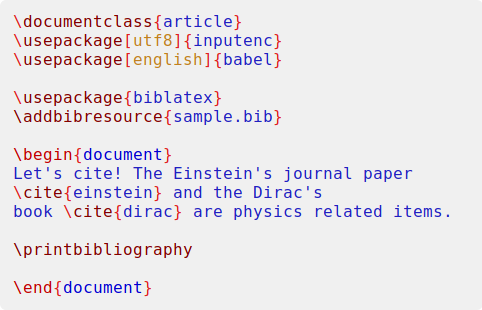
\includegraphics[width=5cm]{/home/ivana/racunalne_bibliografija/prviprimjer.png}
	\end{figure}
\end{itemize}
\end{frame}

\begin{frame}
\begin{itemize}
	\item paket se poziva naredbom \textbackslash usepackage\{biblatex\}\\
	\item \textbackslash cite je naredba kojom dodajemo referencu u tekst dokumenta \\
	\item \textbackslash printbibliography je naredba kojom se ispisuje reference \\
\end{itemize}
\end{frame}

\begin{frame}{Bibtex sintaksa}
\begin{itemize}
	\item prvo se navodi na što se informacija koja se navodi u referenci odnosi \\
	\begin{itemize}
		\item @article\{...\} \\
		\item @book \{...\}\\
		\item @online \{...\} ... \\
	\end{itemize}
	\item ime reference, koristi se u tekstu kada se želi dodati određena referenca \\
	\item autor, naslov, godina... 
		\begin{itemize}
			\item primjer: year = 2010.
		\end{itemize}
\end{itemize}
\end{frame}

\begin{frame}{Parametri}
\begin{itemize}
	\item parametri, odnosno dodatne opcije, dodaju se unutar uglatih zagrada i odvajaju se zarezom \\
	\item može se mijenjati pozadina, stil (redoslijed referenci), način sortiranja... \\
	\item primjer:
	\begin{figure}
		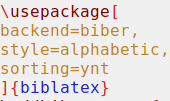
\includegraphics[width=2.5cm]{/home/ivana/racunalne_bibliografija/drugiprimjer.png}
	\end{figure}
\end{itemize}
\end{frame}

\begin{frame}{Dodavanje bibliografije u sadržaj}
\begin{itemize}
	\item dodatne opcije se upisuju pokraj \textbackslash printbibliography \\
	\item primjer:
	\begin{figure}
	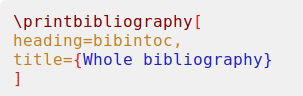
\includegraphics[width=5cm]{/home/ivana/racunalne_bibliografija/treciprimjer.png}
	\end{figure}
\end{itemize}
\end{frame}

\begin{frame}{Zaključak}
\end{frame}

\begin{frame}
Hvala na pažnji!
\end{frame}

\end{document}